% Please use the skeleton file you have received in the
% invitation-to-submit email, where your data are already
% filled in. Otherwise please make sure you insert your
% data according to the instructions in PoSauthmanual.pdf

\documentclass{PoS}
\usepackage{verbatim}
\usepackage{lineno}

          
\title{Searches for high-mass resonances decaying to pairs of bosons using the ATLAS detector}

\ShortTitle{Searches for high-mass resonances}

\author{\speaker{Kirill Grevtsov}, {on behalf of the ATLAS collaboration}\\%\thanks{A footnote may follow.}\\
        Deutsches Elektronen-Synchrotron (DESY), Notkestr. 85, 22607 Hamburg, Germany\\
        E-mail: \email{kirill.grevtsov@cern.ch}}

%\author{Another Author\\
%        Affiliation\\
%        E-mail: \email{...}}
%http://www.ichep2018.org/03_abstract/s31.html#Proceedings
% There is a page limit:
% 
%  - Parallel talk: 4 pages for <20 min, including the title and reference 

\abstract{Several beyond the Standard Model theories predict the existence of new heavy particles decaying into pairs of gauge bosons. This review summarizes the latest ATLAS results on searches for resonances decaying into $W$, $Z$, Higgs bosons or photons, based on datasets of 36  and 80 fb$^{-1}$ of $pp$ collision data collected at 13 TeV. % will be discussed.
No excess of events is found over the Standard Model background-only expectation, exclusion limits are set for various hypotheses in a broad mass range.
}

\FullConference{The 39th International Conference on High Energy Physics (ICHEP2018)\\
		4-11 July, 2018\\
		Seoul, Korea}



\begin{document}
%\linenumbers

\vspace*{-10mm}
\section{Introduction}
\vspace*{-2mm}
The discovery of a Higgs-like particle announced by the ATLAS and CMS collaborations in 2012 \cite{HIGG-2012-27,CMS-HIG-12-028} has been an important milestone in the understanding of the mechanism of electroweak (EW) symmetry breaking. %[3-5].
%3. F. Englert, R. Brout, Broken symmetry and the mass of gauge vector mesons. Phys. Rev. Lett. 13, 321 (1964). https://doi.org/10.1103/ PhysRevLett.13.321
%4. P.W. Higgs, Broken symmetries and the masses of gauge bosons. Phys. Rev. Lett. 13, 508 (1964). https://doi.org/10.1103/ PhysRevLett.13.508
%5. G.S. Guralnik, C.R. Hagen, T.W.B. Kibble, Global conservation laws and massless particles. Phys. Rev. Lett. 13, 585 (1964). https:// doi.org/10.1103/PhysRevLett.13.585
The next step is to figure out whether this particle is the only one or if it is part of an extended Higgs sector as predicted by several extensions of the Standard Model (SM): composite Higgs models, heavy vector triplets and models with warped extra dimensions.
%Diboson vector and tensor resonances are also predicted in several other extensions to the SM, such as in composite Higgs mod- els [9, 10] and models with warped extra dimensions [11?14].


In these proceedings a collection of results is presented where the heavy resonances decay into diboson final states. 
The analyses are separated according to the diboson composition ($W,Z, \gamma$) and the decays of the bosons. 
%A search for additional heavy resonances in diboson final states is presented for several channels.
%Searches for heavy resonances decaying to $WW$ and $ZZ$ with leptonic decays of $W$ and $Z$ bosons are described in Section~\ref{sec:WW} and \ref{sec:ZZ} using 36 fb$^{-1}$ of data.
Searches for heavy resonances decaying to $WW$ with leptonic decays of $W$ bosons are described in Section~\ref{sec:WW} using 36 fb$^{-1}$ of data.
A search for fully hadronic decays of $VV$ ($WW, WZ, ZZ$) is described in Section~\ref{sec:VV} using 80 fb$^{-1}$ of data, results of a search for a photon and a hadronically decaying boson ($Z,W$ or $H$) are presented in Section~\ref{sec:gV} based on a dataset corresponding to an integrated luminosity of 36 fb$^{-1}$. 
The brief overview of searches are summarised in Section~\ref{sec:sum}.

%\newpage
\vspace*{-4mm}
\section{$WW\rightarrow e\nu \mu \nu$ decays}
\label{sec:WW}
\vspace*{-2mm}
The search for a neutral heavy resonance $H$ decaying to $WW$ with a final state of $e\nu \mu \nu$ is described in detail in~\cite{HIGG-2016-31}. 
The search is performed for the production via quark-antiquark annihilation ($q\bar{q}A$), vector-boson fusion (VBF) or gluon-gluon fusion ($ggF$) process covering a mass range from 200 GeV up to 5 TeV for various benchmark models: a Higgs-like scalar in narrow (N) or large (L) width approximation scenarios
% (NWA-LWA, $\Gamma_X$=0-15\%$m_X$), 
\footnote{
The LWA approximation is studied for three hypotheses on the ratio between the resonance width and mass: 1\%, 5\%, and 10\%  }
a two-Higgs-doublet model (2HDM), the Georgi-Machacek (GM) model, a heavy vector triplet model (HVT), a warped extra dimension model predicting  Kaluza-Klein graviton excitations ($G_{KK}$) and an effective Lagrangian model (ELM).

The analysis studies opposite sign, different flavour leptons and categorises events into three signal regions (SR), two VBF enriched and one targeting $ggF$ and $q\bar{q}A$. 
%For each signal region corresponding control region (CR) defined to estimate normalisations for 
The main backgrounds ($t\bar{t}$ and non-resonant $WW$) are estimated with simulations  and normalised using dedicated CRs, while the $W$+jets background was obtained with data-driven techniques. 
%Shapes of main backgrounds are taken from simulation and normalised using dedicated CRs, 
%Due to the presence of large missing energy, discriminant variable is transverse mass ($m_T$), fitted simultaneously in SRs and CRs. 
%Plots shows binned transverse mass distribution for two signal regions, for data and background predictions. 
%Data fitted simultaneously in all the SRs and the CRs - no excess over the background prediction is observed

As no excess over the background prediction is observed, upper limits at 95\% CL$_s$ on $\sigma_H \times B(H\rightarrow WW)$ are set for $ggF$(VBF) in the range of 0.2-4(3) TeV. 
Values above 6.4(1.3) pb at $m_H$=200 GeV and above 0.008(0.006) pb at 4(3) TeV are excluded at 95\% CL by the quasi-inclusive $ggF$(VBF) NWA analysis.
% For the LWA 15\% case, the upper exclusion limit ranges between 5.2 pb (1.3 pb) at m H = 200 GeV and 0.02 pb (0.006 pb) at 4 (3) TeV for the $ggF$(VBF) signals.
%Limits are set for signal widths of 5, 10 and 15\% that are compatible with the NWA one.
Constraints obtained in the LWA approximation, for all values of $\Gamma_X/m_X$ are comparable to those obtained in the NWA case.
The NWA limits are translated into exclusion contours  for Type I and Type II 2HDM in the plane of $tan \beta$ versus $cos(\beta-\alpha)$.
The current sensitivity is not sufficient to exclude the GM signal with masses between 200 GeV and 1 TeV.
Heavy vector triplet signals below about 1.3 TeV are excluded at 95\% CL. 
The observed limits exclude a KK graviton signal lighter than 1.1 TeV (750 GeV) with the $k/\overline{M}_{Pl}$=1(0.5), while the current sensitivity is not sufficient to exclude the ELM spin-2 VBF signal. 

\begin{comment}
\vspace*{-3mm}
\section{$ZZ\rightarrow \ell^+\ell^-\ell^+\ell^-$ and $\ell^+\ell^-\nu\bar{\nu}$ decays} %l+l?l+l?
\label{sec:ZZ}
\vspace*{-2mm}
 Searches for a heavy resonance decaying into two SM $Z$ bosons are performed in the four lepton and two lepton plus two neutrino channels (where lepton stands for either an electron or a muon)~\cite{HIGG-2016-19}, with similar strategies as discussed in Section~\ref{sec:WW}. 
%Searches for a heavy resonance decays into two SM $Z$ bosons are performed in four lepton and two lepton, two neutrino channels (where lepton stands for either an electron or a muon)~\cite{HIGG-2016-19}, with similar strategies as discussed in Section~\ref{sec:WW}. 
The search is performed in a mass range from 200~GeV up to 1.4 TeV for narrow width signals and up to 1 TeV for large width hypothesis in a search for spin-0 resonances. A search for gravitons was done in a mass range extending up to 2 TeV.

The analysis is done selecting two same-flavour, opposite-sign lepton pairs in the $4\ell$ channel and selecting one pair with 120 GeV cut on missing energy associated with escaping neutrinos in $2\ell2\nu$.
Events are classified into categories: VBF or three
\footnote{
 for each of the lepton pair flavour - $\mu\mu$, $e\mu$ and $ee$
 }
 $ggF$.
%Four lepton mass ($m_{4\ell}$) and transverse mass ($m_T$) used as discriminant variables in $4\ell$ and $2\ell2\nu$ channels correspondingly.
%Signal described as CrystalBall+Gaussian (moment-morphing) used to model signal in $4\ell$ ($2\ell2\nu$) channel. 
In the LWA case this search accounts for two interference effects between the heavy scalar and the SM Higgs boson and between the heavy scalar and non-resonant $ZZ$ continuum.
Non resonant $ZZ$ contribution to the background os estimated from simulation, $Z$+jets from data; $t\bar{t}$, $WZ$ and $WW$ are estimated from dedicated CRs.

The largest deviation from the background expectation was found at 700 GeV in the $4\ell$ analysis for $ggF$ corresponding to 3.6(2.2)$\sigma$ local(global), while no significant deviation is observed in $2\ell2\nu$. Combined results are compatible with SM expectations. 
Upper limits on $\sigma_H \times B(H\rightarrow ZZ)$ are set for $ggF$(VBF) in the $m_H$ range 200-1200 GeV, corresponding to 0.68(0.41) pb at $m_H$=240 GeV to 11(13) fb at $m_H$=1200 GeV.
The NWA limits are translated into exclusion limits in the $tan \beta$ versus $cos(\beta-\alpha)$ plane for Type-I and Type-II 2HDM. 
The limits on the production rate of a large-width scalar are obtained for $\Gamma_X/m_X$ of 1, 5 and 10\%. % of the mass of the resonance.
The results are interpreted as a search for a Kaluza-Klein graviton excitation, excluding this signal up to a mass of 1.3 TeV. %, which is consistent to results of the search discussed in Section~\ref{sec:WW}. 

\end{comment}

%\section{Hadronic decays of $WW, WZ$ or $ZZ$ boson pairs}
\vspace*{-4mm}
\section{$VV\rightarrow qqqq$}
\label{sec:VV}
\vspace*{-2mm}
A search for narrow resonances decaying into $WW$, $WZ$ or $ZZ$ boson pairs, with hadronic decays of $V$, is performed with 80 fb$^{-1}$ as described in~\cite{ATLAS-CONF-2018-016}. The search covers diboson resonances with masses in the range of 1.2-5.0 TeV for two specific benchmark models: a spin-1 HVT model with signals such as $W'$ and $Z'$ and a spin-2 Kaluza-Klein graviton.

Bosons produced in the decay of TeV-scale resonances are highly boosted and therefore are reconstructed in ATLAS as a single large radius parameter jet. 
This analysis uses a new unified object built from both tracking and calorimeter information, referred to as Track-CaloCluster~\cite{ATL-PHYS-PUB-2017-015}. 
Jet substructure and mass are exploited to enhance the separation between signal boson jets and jets from multijet background. 
%Optimised tagger Boson jet mass presented as a function of jet pT. 
The efficiency of the boson tagger is determined in a $V$+jet CR, by fitting the jet mass distribution after applying jet substructure cut. % as presented on the plot.
After boson-tagging, the data is categorised in five non-exclusive signal regions with different signal efficiencies.
The signal model is taken from simulation and background parametrised with functional form. 
The modelling of the parametric shape tested in a dedicated fit control region in data.
%Comparison of the dijet mass distributions of the selected events in the combined signal regions with the expected background distribution from the background-only fits to the data. 

A signal-plus-background fit is performed on the discriminant distribution $m_{JJ}$.
No significant deviation is found, therefore upper limits on the production cross section times branching ratio to diboson final states for new resonances with masses between 1.2 and 5.0 TeV are set at the 95\% CL, excluding the production of $WW+WZ$ from the HVT model A(B), with $g_V$=1(3) and masses in the range of 1.20-3.40(1.20-4.15) TeV. 
Production of a $G_{KK}$ in the bulk RS model with $k/\overline{M}_{Pl}$=1 is excluded in the range of 1.20-1.90 TeV and 2.1-2.3 TeV, at the 95\% CL.

%\section{Resonances decaying to a $Z$, $W$, or Higgs boson and a photon}
\vspace*{-4mm}
\section{$Z/W/H+\gamma$ hadronic decays}
\label{sec:gV}
\vspace*{-2mm}
A search for resonance decays to a photon and a $Z$, $W$ or Higgs boson with subsequent hadronic decay of these bosons is presented and discussed in details in Ref.~\cite{EXOT-2016-30}. 
Searches for $Z\gamma$ ($W\gamma$) are carried out in the mass range of 1.0-6.8 TeV for spin-0 and 2 (spin-1) signals and for $H\gamma$ in the range of 1.0-3.0 TeV for spin-1 signal in the $q\bar{q}A$ channel.

This analysis looks for energetic photons and boosted bosons reconstructed as one large jet.
Events are classified into four categories to improve the expected signal sensitivity, presented by different signal efficiency. 
The separation is based on exploiting $b$-tagging for $Z$ and Higgs to $b\bar{b}$ (BTAG), cuts on jet substructure (D2) and jet mass window (VMASS) to separate hadronically decaying bosons from quark-gluon initiated jets.
The signal is modelled by CrystalBall+gaussian, and the background is modelled as a functional form using spurious signal as uncertainty. $\gamma$+jet and SM $\gamma V$ are taken from simulation and multijet is estimated from data-driven tecnhiques.
The jet-photon mass distribution ($m_{J \gamma}$) are used as a discriminant variable. %for selected in BTAG category presented for data and overlaid  background-only fit and signal on top.

The largest deviation from the SM expectation, corresponding to a significance of 2.7$\sigma$, is found in the $W\gamma$ search at $m_{J \gamma}$=2.5 TeV.
In the absence of any significant excess, limits are set on hadronic $W$ boson decays.
The limit varies from about 10 fb at $m_X$=1.0 TeV to 0.1 fb for 6.6 TeV. %, as shown on the left at Figure~\ref{fig:Wg_lim}. 
%This is the first search for a heavy resonance in $H\gamma$ with this decay mode.
The limit on $H\gamma$ production is evaluated for resonance masses between 1 and 3 TeV and varies between 10 fb and 4 fb depending on $m_X$.
The limits on $Z\gamma$ production, vary from about 10 fb to 0.1 fb, for $m_X$ between 1.0 and 6.8 TeV, for spin-0 and spin-2 hypothesis. % for $ggF$ and $q\bar{q}A$.
%\vspace*{-4mm}
% \begin{figure}
% \hspace{5mm}
%     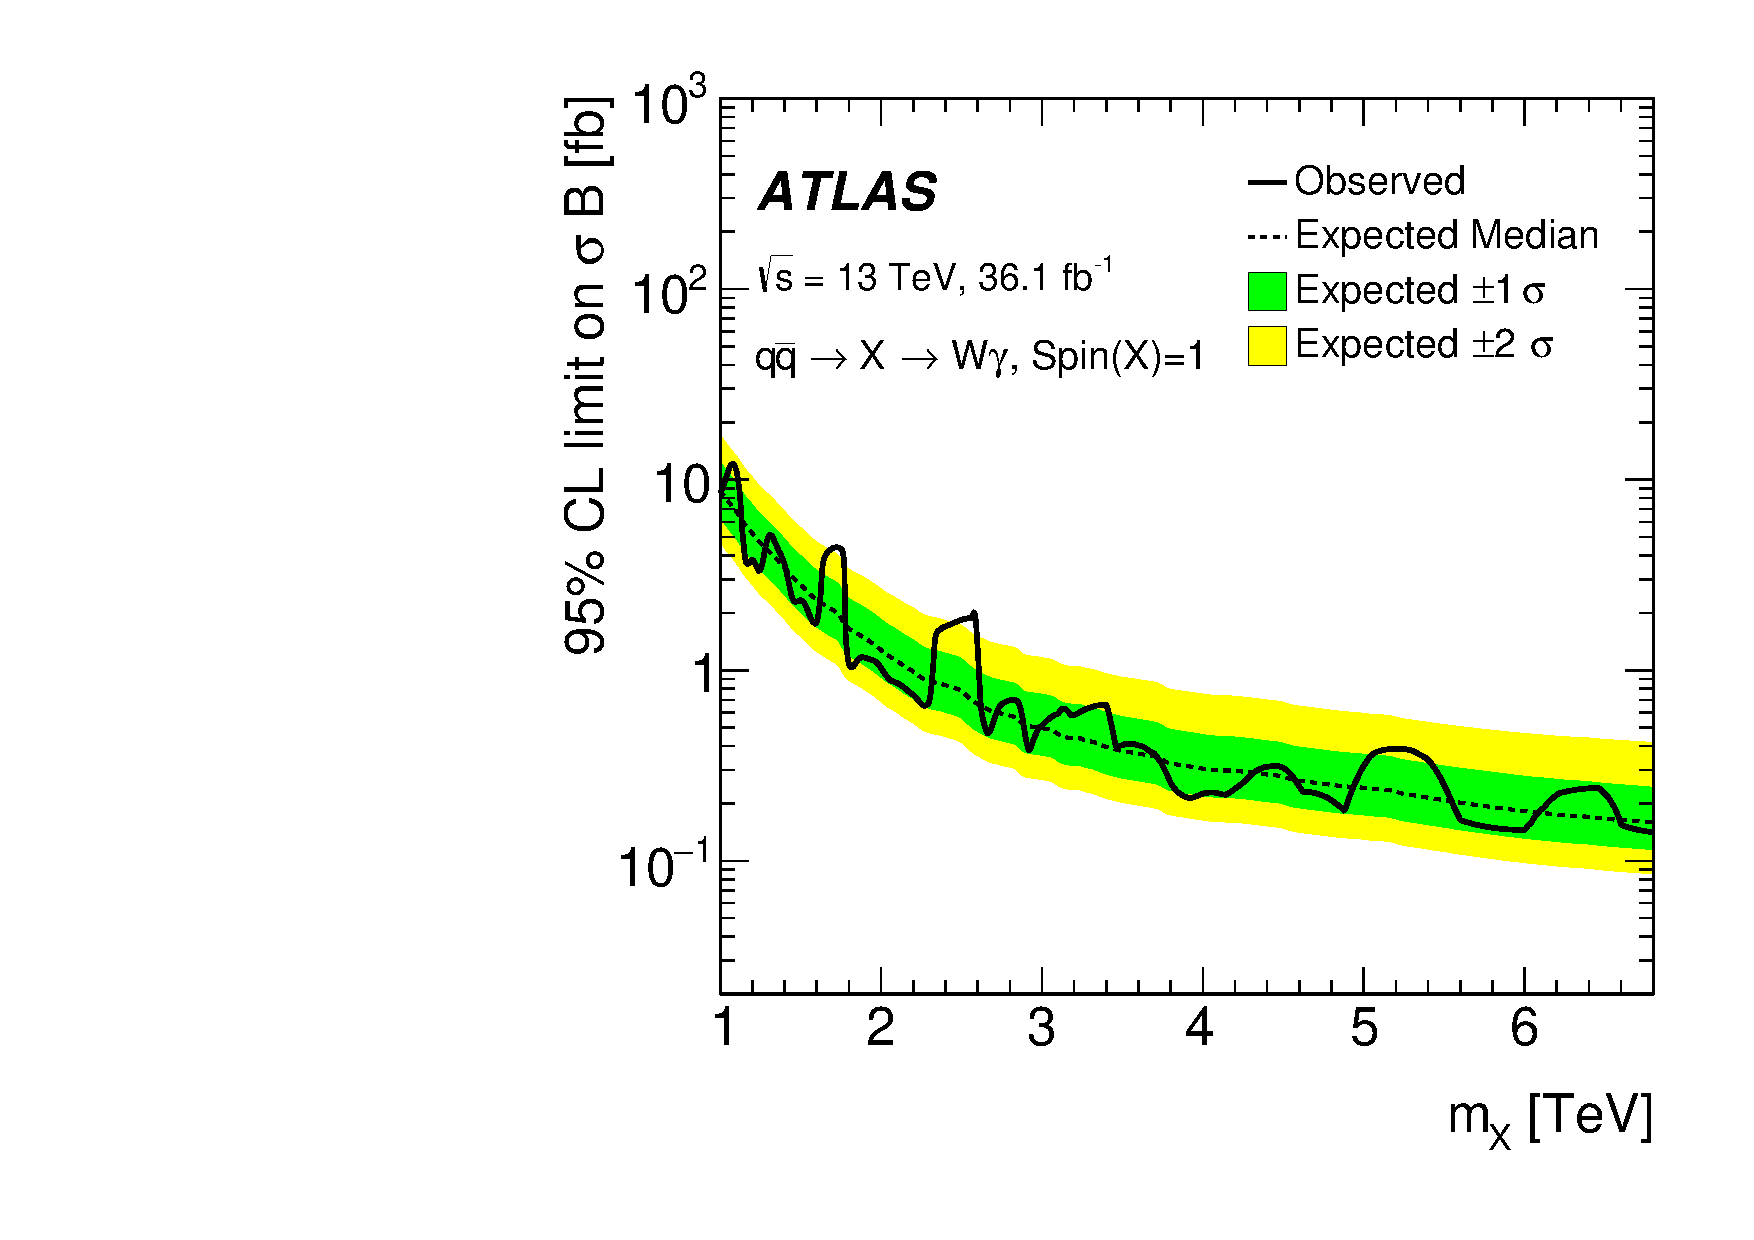
\includegraphics[width=.4\textwidth]{figures/lim_Wg_qqA1}
% \hspace{10mm}
%      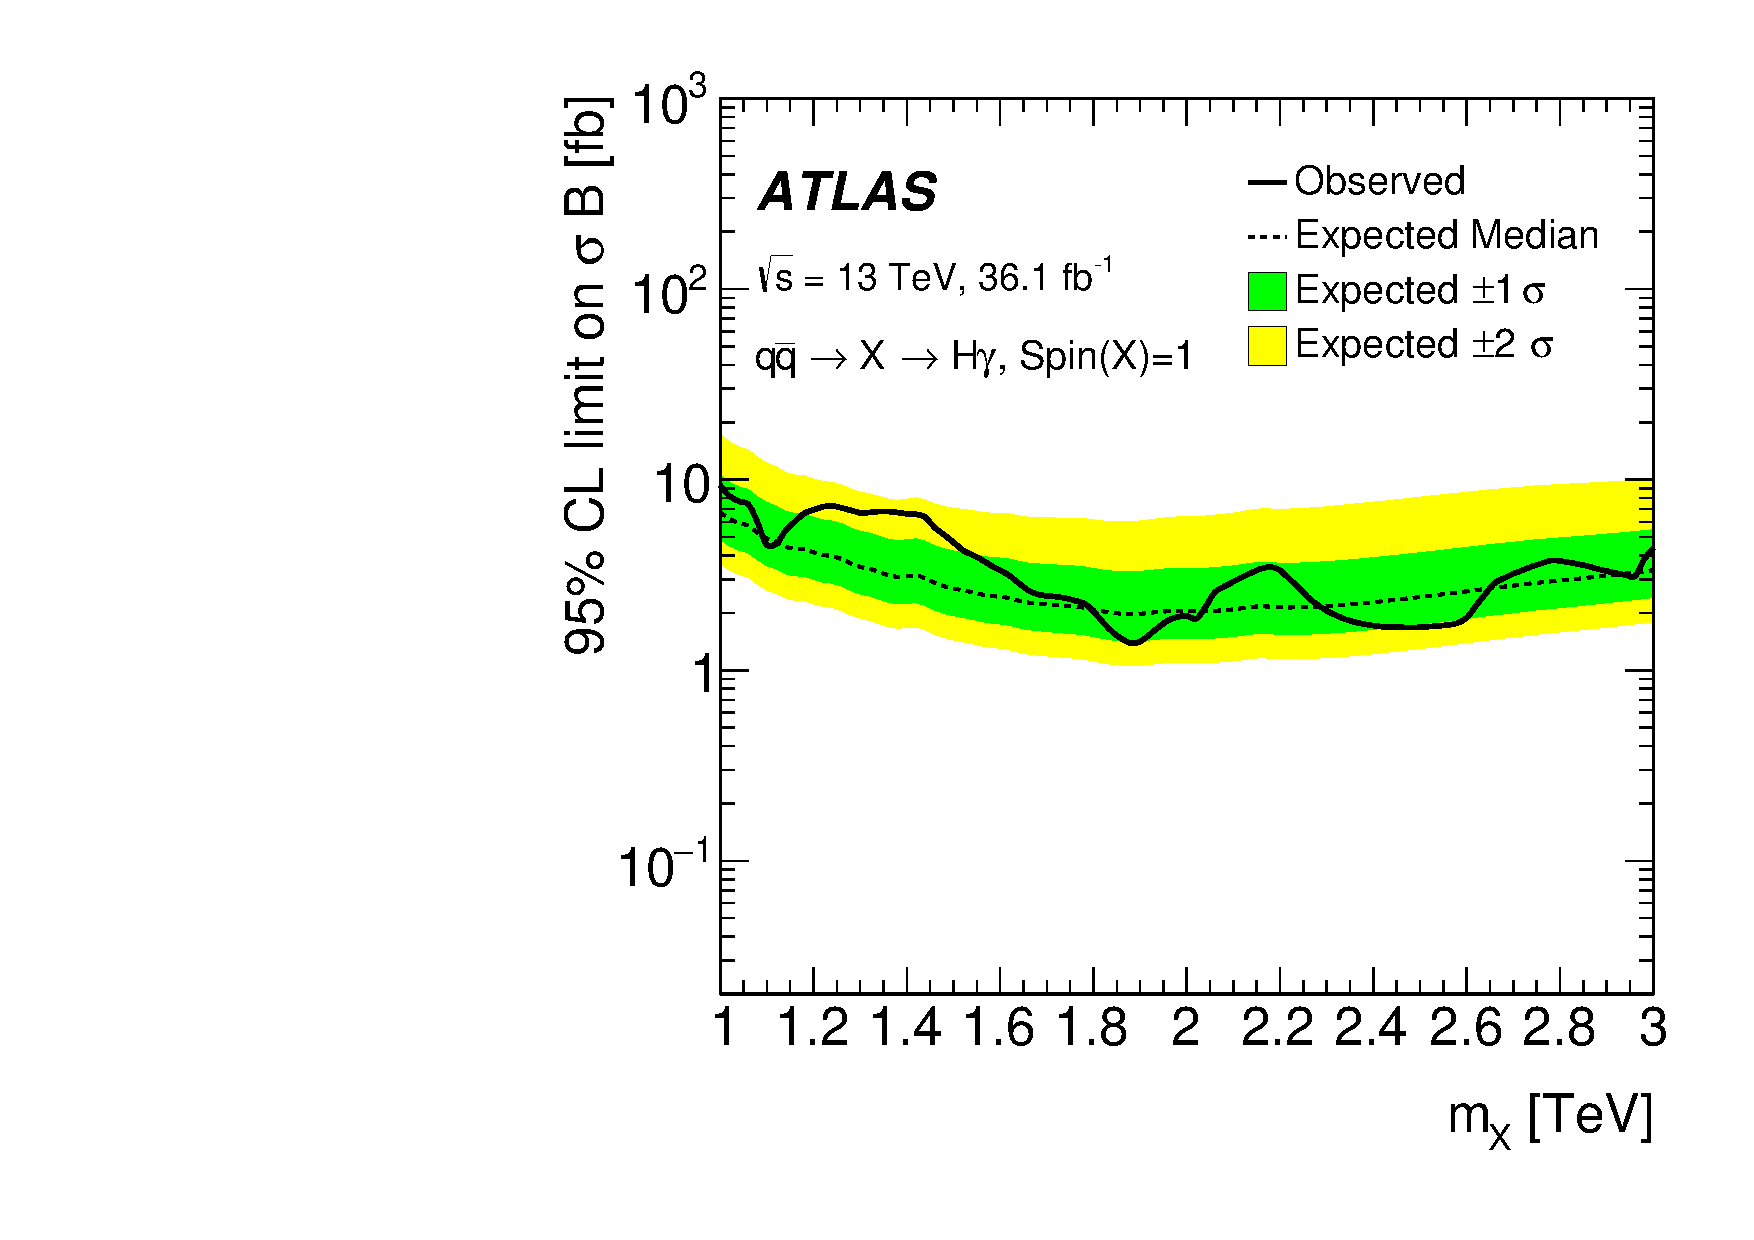
\includegraphics[width=.4\textwidth]{figures/lim_Hg_qqA1}
%      \vspace*{-2mm}
%     \caption{The 95\% CL observed (solid line) and expected (dashed line) upper limits on $\sigma B$ for a spin-1 resonance decaying to $W\gamma$ (left) and $H\gamma$ (right), as a function of the resonance mass~\cite{EXOT-2016-30}.}
%     \label{fig:Wg_lim}
%     \end{figure}
%\vspace*{-10mm}

\vspace*{-4mm}
\section{Summary}
\label{sec:sum}
\vspace*{-2mm}
The ATLAS Collaboration has performed a rich search program for additional heavy resonances decaying into two bosons in various final states, testing several benchmark models.
The searches presented in this review used datasets collected in $pp$ collisions at $\sqrt{s}$=13 TeV corresponding to 36 and 80 fb$^{-1}$.
No excess of events over the SM expectation was found in any of the final states taken into account. 
Figure~\ref{fig:summary} presents a sketch, combining a variety of upper limits set on the collection of diboson channels, covering various spin hypotheses and a broad mass range from 200 GeV up to 6.8 TeV.
%The right plot on Figure~\ref{fig:summary} presents total luminosity collected by atlas in Run-2, which shows doubled dataset with respect to studied so far.

  \begin{figure}
    \begin{center} 
\vspace*{-5mm}
    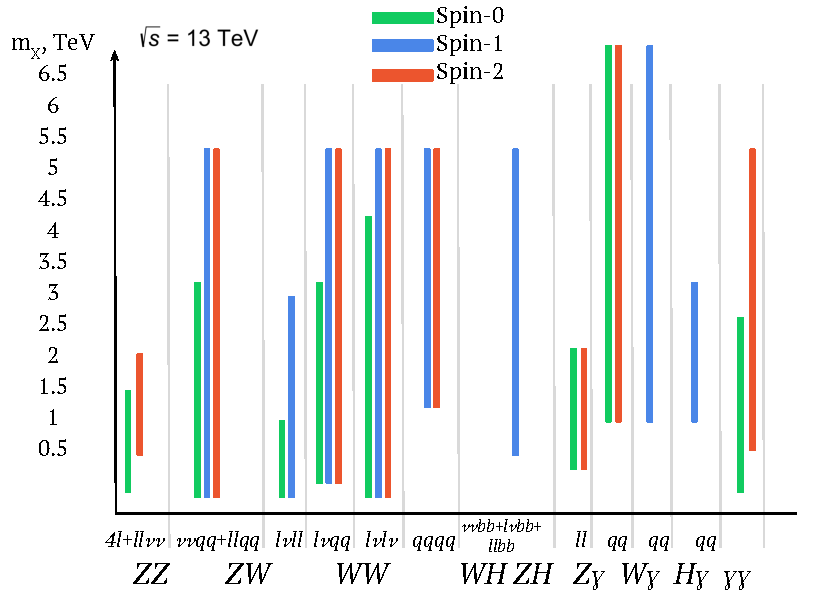
\includegraphics[width=.5\textwidth]{figures/lim_sketch}
    \end{center}
     %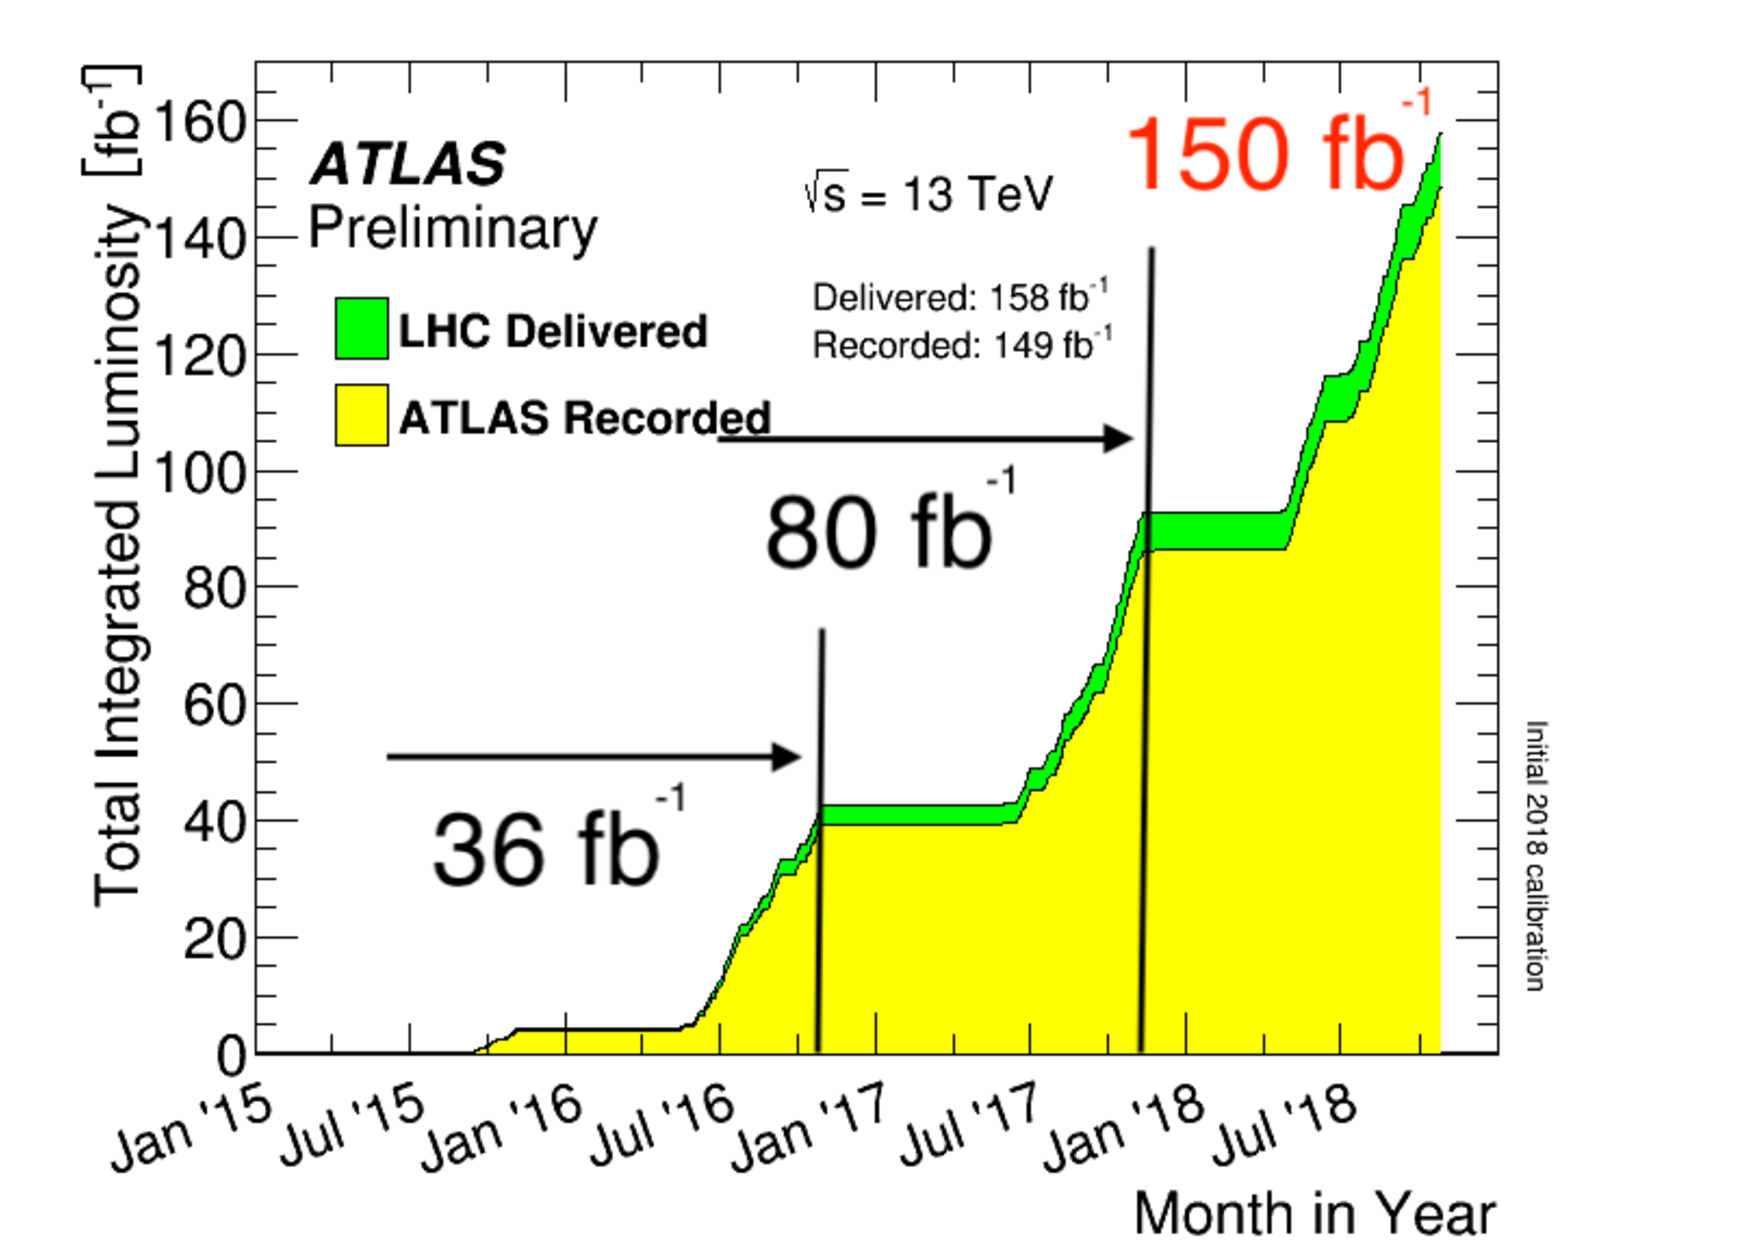
\includegraphics[width=.5\textwidth]{figures/intlumivstimeRun2}
     %\caption{Left: combination of limits set on various diboson channels, covering large mass range and spin hypothesis. Right: cumulative luminosity versus time recorded by ATLAS (yellow).}
\vspace*{-8mm}
     \caption{Combining upper limits set on various diboson channels, covering a broad mass range and spin hypotheses - graphical representation of results published in \cite{HIGG-2016-31,HIGG-2016-19,ATLAS-CONF-2018-016,EXOT-2016-30,EXOT-2016-29,EXOT-2016-28,HIGG-2016-17,EXOT-2016-10-2}}
     \label{fig:summary}
     \end{figure}

\vspace*{-6mm}
%\printbibliography
\bibliographystyle{JHEP}
%\begin{thebibliography}{99}
\bibliography{all.bib}
%\bibliography{bib/CMS.bib}
%\bibitem{test}
%ATLAS collaboration, G. Aad et al., \textit{Observation of a new particle in the search for the Standard Model Higgs boson with the ATLAS detector at the LHC, Phys. Lett.} B716 (2012) 1-29, [1207.7214].
%%%
%\end{thebibliography}

\end{document}
